% Shared preamble for the English summaries in this repository.
\documentclass[11pt,a4paper]{article}
\usepackage[margin=2.2cm]{geometry}
\usepackage[T1]{fontenc}
\usepackage[utf8]{inputenc}
\usepackage{lmodern}
\usepackage{amsmath,amssymb}
\usepackage{graphicx}
\usepackage{booktabs}
\usepackage{enumitem}
\usepackage[hidelinks]{hyperref}
\setlist{itemsep=2pt,topsep=4pt}
\setlength{\parindent}{0pt}
\setlength{\parskip}{5pt}
\graphicspath{{figures/}}
\newcommand{\summaryheader}[3]{%
  \begin{center}
    {\Large\bfseries #2}\\[3pt]
    {\large #1}\\[3pt]
    {\small Arshia Goshtasbi \textbullet{} MSc Electrical Engineering (Control), Iran University of Science and Technology \textbullet{} #3}
  \end{center}
  \vspace{2pt}\hrule\vspace{8pt}
  \noindent\textit{English summary of my original Persian report, which is kept as a PDF in this folder.}\par}

\begin{document}
\summaryheader{Optimal Control, Homework 5}{Tracking LQR with Riccati and Feed-forward Equations (Kirk Examples 5.2-3 and 5.2-4)}{Spring 1404 (2025)}

Both examples are linear tracking problems on the same second-order plant. The optimal control is $u^\star(t)=-R^{-1}B^T[K(t)x(t)+s(t)]$. Besides the Riccati equation for $K(t)$, a second linear equation for the feed-forward vector $s(t)$ is integrated backwards from the final time.

\section*{Example 5.2-3 (\texttt{Q5\_2\_3.slx})}
\texttt{Q5\_2\_3\_Gains.m} integrates five equations ($K_{11}$, $K_{12}$, $K_{22}$, $s_1$, $s_2$) backwards from $t_f=15$\,s with \texttt{ode45}, using the terminal values from the book. The control law is in a MATLAB Function block (\texttt{myfcn}). My report notes that the curves match the book.
\begin{center}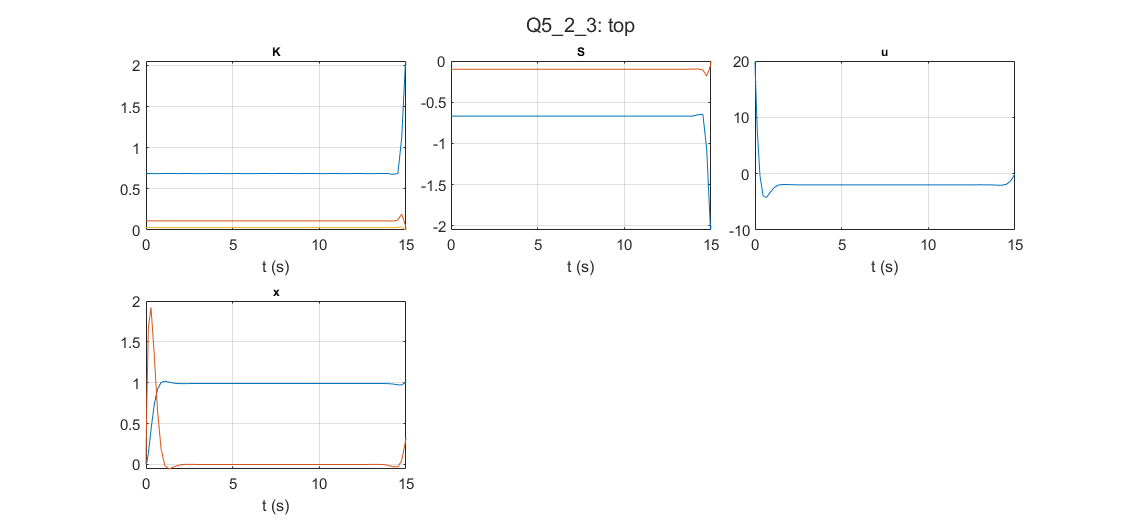
\includegraphics[width=0.7\linewidth]{Q5_2_3_scopes.png}\end{center}

\section*{Example 5.2-4 (\texttt{Q5\_2\_4.slx})}
This case has a time-varying reference: the $s_1$ equation has a $0.4t$ forcing term and zero terminal conditions. The structure of the model is the same.
\begin{center}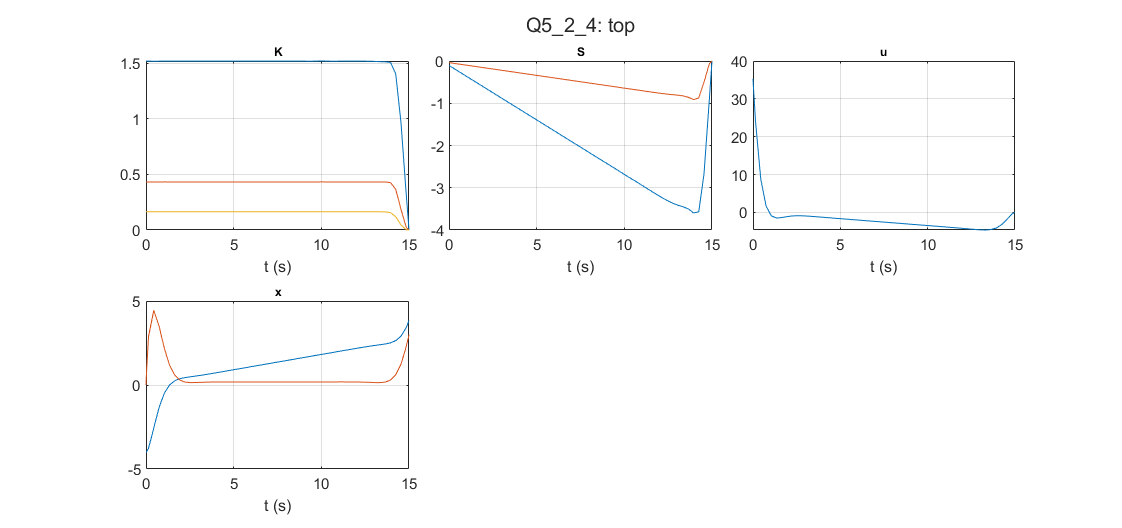
\includegraphics[width=0.7\linewidth]{Q5_2_4_scopes.png}\end{center}

\textit{How to run:} run the matching \texttt{*\_Gains.m} script first, then the model.
\end{document}
